\documentclass[11pt,a4paper]{article}

\usepackage[utf8]{inputenc}
\usepackage[T1]{fontenc}
\usepackage[french]{babel}
\usepackage{lmodern}
\usepackage{microtype}
\usepackage[margin=2.3cm]{geometry}
\usepackage{booktabs}
\usepackage{tabularx}
\usepackage{array}
\usepackage{xcolor}
\usepackage{enumitem}
\usepackage{float}
\usepackage{graphicx}
\usepackage{amsmath}
\usepackage{pifont}
\usepackage[round,authoryear]{natbib}
\usepackage[colorlinks=true,linkcolor=teal!70!black,citecolor=teal!70!black,urlcolor=teal!70!black]{hyperref}

\newcolumntype{Y}{>{\raggedright\arraybackslash}X}
\newcommand{\oui}{\textcolor{teal!70!black}{\ding{51}}}
\newcommand{\non}{\textcolor{red!60!black}{\ding{55}}}
\setlist{itemsep=2pt,topsep=4pt}

\title{\textbf{Livrable L5 -- Évaluation finale}\\[4pt]
\large Allocation adaptative des ressources de calcul et de recherche documentaire\\ pour des systèmes LLM locaux, économes et fiables\\[2pt]
\normalsize\textit{Exécution unique sur le jeu de test, verdict sur les critères pré-enregistrés, ablations et énergie}}
\author{Alae Lahbichi -- Étudiant en 5\textsuperscript{e} année IA/Data\\[2pt]
\small\href{mailto:a.lahbichi2004@gmail.com}{\texttt{a.lahbichi2004@gmail.com}}\\
\small Dépôt GitHub : \href{https://github.com/AlaeLahbichi/Adaptive-Compute-and-RAG-for-Efficient-Reliable-Local-LLMs}{\footnotesize\texttt{AlaeLahbichi/Adaptive-Compute-and-RAG-for-Efficient-Reliable-Local-LLMs}}}
\date{18 octobre 2026}

\begin{document}
\maketitle

\begin{abstract}
\noindent La politique adaptative figée en Partie IV a été exécutée une seule fois sur les 450 questions du jeu
de test, avec les six stratégies fixes, les routeurs de référence R1 et R2 et une mesure d'énergie. Sa
\textbf{qualité est au niveau de la référence B} (score global 0,550 contre 0,537, soit +1,3~point ;
intervalle à 95~\% de la perte : $[-4{,}1\,;\,+1{,}6]$~points, donc non-infériorité démontrée) et elle
\textbf{bat les deux routeurs de référence} (R1 : 0,489 ; R2 : 0,517). En revanche, elle ne réduit la
latence moyenne que de \textbf{10~\%} (0,79~s contre 0,87~s), loin des 20~\% exigés, et l'énergie par
question de 9~\%. \textbf{Le critère de succès principal n'est donc pas atteint.} La cause est
identifiée : l'abstention précoce, réglée sur 180 questions, se déclenche sur 25~\% des questions de
développement mais seulement sur 15~\% des questions de test. Le critère de robustesse échoue aussi
(perte de 7,6~points sur les questions simples).
\end{abstract}

\clearpage
\tableofcontents
\clearpage

%======================================================================
\section{Rôle de cette partie}
%======================================================================

Les Parties II à IV ont fixé le protocole (\texttt{protocole-v1.0}), construit les méthodes de référence
et réglé la politique adaptative (\texttt{politique-v1.0}), le tout sur le jeu de développement. La
Partie V applique \emph{une seule fois} toutes les méthodes aux 450 questions du jeu de test, jamais
utilisées jusque-là, et confronte les résultats aux critères de succès écrits avant les expériences
(L2, section 8). C'est la seule mesure non biaisée de l'étude.

%======================================================================
\section{Déroulement}
%======================================================================

\begin{itemize}
\item \textbf{Méthodes exécutées} : les six stratégies fixes (A à F) et la politique adaptative,
exécutée réellement de bout en bout. Les routeurs de référence R1 et R2, entraînés sur le jeu de
développement avec les réglages de la Partie III, sont appliqués aux sorties des stratégies sur le test.
L'oracle est calculé de la même manière.
\item \textbf{Trois passes complètes}, conformément au protocole : la latence retenue pour chaque
question est la médiane des trois passes ; la qualité provient de la première passe, la génération
étant déterministe. Dans chaque passe, l'ordre des méthodes est tiré au hasard (graine fixe) pour
répartir l'effet de l'échauffement de la machine.
\item \textbf{Énergie} mesurée par \texttt{powermetrics} pendant toute l'évaluation (puissance CPU + GPU
+ ANE, toutes les 200~ms), après 20~s de mesure au repos. L'énergie par question inclut les 3 requêtes
de chauffe de chaque méthode dans le dénominateur.
\item \textbf{Aucun réglage} n'a été modifié après l'exécution sur le test.
\end{itemize}

\paragraph{Bilan de l'exécution.} 9\,450 sorties ont été produites (7 méthodes $\times$ 450 questions
$\times$ 3 passes) en environ 2~h. Deux contrôles valident l'exécution :
\begin{itemize}
\item \textbf{Stabilité} : pour toutes les méthodes, les trois passes donnent exactement la même réponse
sur 100~\% des questions ; seule la latence varie.
\item \textbf{Fidélité de la simulation} : rejouer la politique à partir des sorties des stratégies fixes
(comme lors du réglage en Partie IV) reproduit son score sur 100~\% des questions (0,550) et sa latence
à 0,001~s près (0,786~s simulée contre 0,786~s mesurée). Le réglage par simulation de la Partie IV
était donc exact.
\end{itemize}

%======================================================================
\section{Verdict sur les critères pré-enregistrés}\label{sec:verdict}
%======================================================================

Le tableau~\ref{tab:verdict} reprend un à un les critères écrits dans le cahier expérimental (L2)
avant toute expérience.

\begin{table}[H]
\centering\small
\begin{tabularx}{\linewidth}{Y >{\centering\arraybackslash}p{5.6cm} c}
\toprule
Critère pré-enregistré & Mesure sur le test & Atteint \\
\midrule
\textbf{Principal} -- latence moyenne réduite d'au moins 20~\% par rapport à B & $-10{,}1$~\% (0,786 contre 0,873~s) & \non \\
\textbf{Principal} -- perte de score global $\le 2$~points & $-1{,}3$~point (gain) & \oui \\
Non-infériorité : borne haute de l'IC à 95~\% de la perte $< 2$~points & $[-4{,}1\,;\,+1{,}6]$ & \oui \\
\midrule
\textbf{Critère principal (les deux conditions)} & & \non \\
\midrule
Risque (erreurs parmi les réponses données) inférieur à B & 0,395 contre 0,421 & \oui \\
Meilleur score que R1 (routeur « question seule ») & 0,550 contre 0,489 & \oui \\
Meilleur score que R2 (Adaptive-RAG simplifié) & 0,550 contre 0,517 & \oui \\
Robustesse : aucune catégorie ne perd plus de 5~points & simple $-7{,}6$ ; complexe $-3{,}3$ ; non couverte $+14{,}7$ & \non \\
\bottomrule
\end{tabularx}
\caption{Verdict sur les critères de succès pré-enregistrés (jeu de test, 450 questions). Les intervalles
sont obtenus par bootstrap apparié (10\,000 tirages).}
\label{tab:verdict}
\end{table}

\paragraph{Conclusion.} L'hypothèse principale est \textbf{rejetée dans sa forme pré-enregistrée} : la
politique conserve la qualité de B, avec moins d'erreurs, mais n'économise que la moitié de la latence
visée. Le résultat positif est réel mais plus modeste : à qualité égale (non-infériorité démontrée), la
politique est 10~\% plus rapide et 9~\% plus économe en énergie que B, et elle domine les deux routeurs
de la littérature reproduits ici, qui sont à la fois moins bons et, pour R2, à peine plus rapides.

%======================================================================
\section{Résultats détaillés}\label{sec:resultats}
%======================================================================

\begin{table}[H]
\centering\small\setlength{\tabcolsep}{4pt}
\begin{tabular}{l c c c c c c c}
\toprule
Méthode & Score & IC 95~\% & Écart à B & Latence & P95 & Couv. & Risque \\
\midrule
A -- grand, sans RAG & 0,310 & [0,269 ; 0,351] & $-22{,}7$ & 0,27~s & 0,52~s & 0,45 & 0,76 \\
\textbf{B -- grand, 3 passages (réf.)} & \textbf{0,537} & [0,494 ; 0,581] & -- & \textbf{0,87~s} & 1,26~s & 0,73 & 0,42 \\
C -- petit, sans RAG & 0,223 & [0,187 ; 0,261] & $-31{,}4$ & 0,13~s & 0,25~s & 0,51 & 0,93 \\
D -- petit, 3 passages & 0,414 & [0,372 ; 0,457] & $-12{,}3$ & 0,35~s & 0,53~s & 0,88 & 0,57 \\
E -- grand, 6 passages & 0,567 & [0,523 ; 0,610] & $+3{,}0$ & 1,57~s & 2,23~s & 0,75 & 0,40 \\
F -- petit, 6 passages & 0,398 & [0,357 ; 0,440] & $-13{,}9$ & 0,61~s & 0,87~s & 0,94 & 0,60 \\
\midrule
R1 -- question seule & 0,489 & [0,445 ; 0,534] & $-4{,}7$ & 0,74~s & 1,61~s & 0,68 & 0,48 \\
R2 -- Adaptive-RAG simplifié & 0,517 & [0,473 ; 0,561] & $-2{,}0$ & 0,82~s & 1,39~s & 0,68 & 0,44 \\
\textbf{Politique adaptative} & \textbf{0,550} & [0,505 ; 0,594] & $\mathbf{+1{,}3}$ & \textbf{0,79~s} & 1,38~s & 0,64 & \textbf{0,40} \\
\midrule
\textit{Oracle} & \textit{0,797} & [0,762 ; 0,831] & $+26{,}0$ & \textit{0,36~s} & 1,09~s & 0,64 & 0,18 \\
\bottomrule
\end{tabular}
\caption{Résultats sur le jeu de test (450 questions). Latence : moyenne par question de la médiane des
trois passes. Couv. : part des questions auxquelles la méthode répond ; risque : part de réponses
fausses parmi elles.}
\label{tab:resultats}
\end{table}

\begin{figure}[H]
\centering
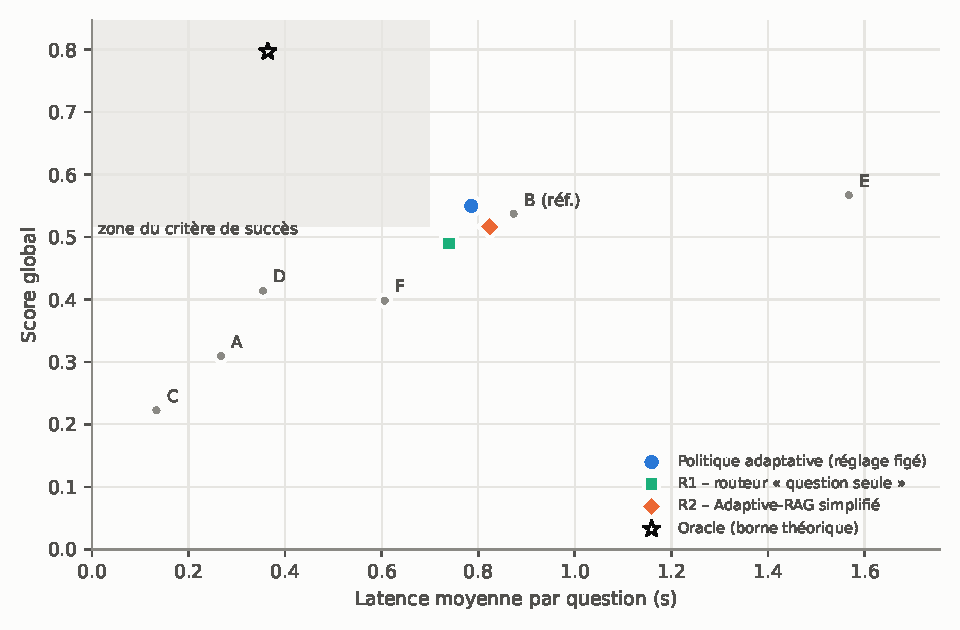
\includegraphics[width=0.82\linewidth]{figures/partie5_qualite_cout.pdf}
\caption{Compromis qualité--latence sur le jeu de test. La zone grisée est celle du critère de succès
(latence $\le 0{,}8\times$B, perte $\le 2$~points). La politique adaptative (en bleu) est au-dessus de B
mais à droite de la zone.}
\label{fig:qualite-cout}
\end{figure}

\paragraph{Par catégorie.} Le tableau~\ref{tab:categories} montre que la politique échange de la
qualité sur les questions qui ont une réponse contre de la fiabilité sur les questions sans réponse.

\begin{table}[H]
\centering\small
\begin{tabular}{l c c c}
\toprule
Méthode & Simple & Complexe & Non couverte \\
\midrule
B -- référence & 0,737 & 0,468 & 0,407 \\
E -- grand, 6 passages & 0,730 & 0,537 & 0,433 \\
R1 & 0,562 & 0,453 & 0,453 \\
R2 & 0,635 & 0,455 & 0,460 \\
\textbf{Politique adaptative} & 0,661 ($-7{,}6$) & 0,435 ($-3{,}3$) & \textbf{0,553} ($+14{,}7$) \\
\textit{Oracle} & 0,842 & 0,682 & 0,867 \\
\bottomrule
\end{tabular}
\caption{Score par catégorie (150 questions chacune). Entre parenthèses : écart de la politique à B, en points.}
\label{tab:categories}
\end{table}

\paragraph{Choix de la politique.} Sur 450 questions : 66 abstentions précoces (15~\%), 359 réponses du
grand modèle avec 3 passages et 25 avec 6 passages ; parmi ces 384 réponses, 98 ont ensuite été
remplacées par une abstention finale. L'abstention précoce touche surtout les questions non couvertes
(36 sur 150), mais aussi 18 questions simples et 12 complexes, ce qui explique la perte sur ces
catégories. Le grand modèle à 6 passages n'est choisi que pour 6~\% des questions : la recherche
adaptative joue un rôle mineur.

%======================================================================
\section{Ablations}\label{sec:ablations}
%======================================================================

Les variantes de la politique, réglées sur le jeu de développement en Partie IV, sont appliquées
au test par simulation (dont la fidélité est vérifiée ci-dessus).

\begin{table}[H]
\centering\small
\begin{tabularx}{\linewidth}{Y c c c c}
\toprule
Variante & Score (test) & Latence (test) & Score (dev) & Latence (dev) \\
\midrule
\textbf{Politique complète} & \textbf{0,550} & 0,79~s & 0,552 & 0,71~s \\
Sans cascade (identique : la cascade n'est pas retenue) & 0,550 & 0,79~s & 0,552 & 0,71~s \\
Sans recherche adaptative (toujours 3 passages) & 0,547 & 0,74~s & 0,548 & 0,68~s \\
Sans abstention finale & 0,547 & 0,79~s & 0,546 & 0,71~s \\
Sans abstention précoce (cascade petit $\to$ grand) & 0,464 & 0,64~s & 0,395 & 0,70~s \\
Sans aucune abstention & 0,457 & 0,64~s & 0,389 & 0,70~s \\
\bottomrule
\end{tabularx}
\caption{Ablations. Chaque variante a été réglée sur le développement sous la même contrainte de latence.}
\label{tab:ablations}
\end{table}

\begin{itemize}
\item Les conclusions de la Partie IV se confirment : \textbf{l'abstention précoce fondée sur la qualité
des preuves est la composante essentielle} ($-8{,}6$~points sans elle).
\item La recherche adaptative (3 ou 6 passages) et l'abstention finale n'apportent chacune que
0,3~point, dans le bruit statistique. Sur le test, \emph{toujours} utiliser 3 passages serait même plus
rapide (0,74~s, soit $-15$~\% par rapport à B) pour un score équivalent.
\item Aucune variante n'atteint à la fois $-20$~\% de latence et une perte $\le 2$~points.
\end{itemize}

%======================================================================
\section{Énergie}\label{sec:energie}
%======================================================================

L'énergie a été mesurée par \texttt{powermetrics} sur toute l'évaluation (30\,630 relevés ; puissance
au repos : 2,7~W). Le tableau~\ref{tab:energie} donne la moyenne des trois passes.

\begin{table}[H]
\centering\small
\begin{tabular}{l c c c}
\toprule
Méthode & Énergie / question & Écart à B & Puissance moyenne \\
\midrule
C -- petit, sans RAG & 1,8~J & $-90$~\% & 16,4~W \\
A -- grand, sans RAG & 3,9~J & $-80$~\% & 17,0~W \\
D -- petit, 3 passages & 7,3~J & $-62$~\% & 23,2~W \\
F -- petit, 6 passages & 13,5~J & $-30$~\% & 24,9~W \\
\textbf{Politique adaptative} & \textbf{17,5~J} & $\mathbf{-9}$~\% & 24,8~W \\
B -- grand, 3 passages (réf.) & 19,3~J & -- & 24,7~W \\
E -- grand, 6 passages & 37,7~J & $+95$~\% & 26,4~W \\
\bottomrule
\end{tabular}
\caption{Énergie (CPU + GPU + ANE) par question sur le jeu de test.}
\label{tab:energie}
\end{table}

La puissance appelée varie peu (16 à 26~W) : l'énergie est presque proportionnelle à la durée de
calcul, donc aux tokens traités. L'économie d'énergie de la politique ($-9$~\%) suit sa réduction de
latence ($-10$~\%). Passer de 3 à 6 passages double l'énergie pour 3~points de score.

%======================================================================
\section{Comparaison avec le jeu de développement}\label{sec:dev-test}
%======================================================================

\begin{table}[H]
\centering\small
\begin{tabular}{l c c c c}
\toprule
& \multicolumn{2}{c}{Développement (180)} & \multicolumn{2}{c}{Test (450)} \\
Méthode & Score & Latence & Score & Latence \\
\midrule
B -- référence & 0,541 & 0,92~s & 0,537 & 0,87~s \\
Politique (réglage figé, estimation optimiste) & 0,552 & 0,71~s ($-23$~\%) & 0,550 & 0,79~s ($-10$~\%) \\
Politique (validation croisée sur dev) & 0,520 & $-22$~\% & -- & -- \\
R1 & 0,425 & 0,74~s & 0,489 & 0,74~s \\
R2 & 0,522 & 0,85~s & 0,517 & 0,82~s \\
Oracle & 0,762 & 0,40~s & 0,797 & 0,36~s \\
\midrule
Abstentions précoces de la politique & \multicolumn{2}{c}{45 / 180 (25~\%)} & \multicolumn{2}{c}{66 / 450 (15~\%)} \\
\bottomrule
\end{tabular}
\caption{Développement et test.}
\label{tab:dev-test}
\end{table}

\begin{itemize}
\item \textbf{La qualité s'est bien généralisée}, mieux même que ne le prévoyait la validation croisée
(0,550 au lieu de 0,520) : la sélection du réglage n'a pas sur-ajusté le score.
\item \textbf{Le gain de latence ne s'est pas généralisé.} Le seuil d'abstention précoce (preuve BM25
normalisée $< 0{,}265$) a été réglé sur 60 questions par catégorie : il coupait 25~\% des questions de développement, mais la
même valeur ne coupe que 15~\% des questions de test (écart d'environ trois erreurs-types, attribuable
à la variabilité d'échantillonnage d'un petit jeu de réglage). Moins d'abstentions précoces signifie plus d'appels au grand modèle, donc une
latence plus proche de B. La validation croisée, faite sur le même petit échantillon, n'a pas pu
révéler ce problème.
\item Le compromis par catégorie garde le même sens (pertes sur les questions simples, gain sur les
questions non couvertes) mais avec une ampleur réduite de moitié, cohérente avec la baisse du taux
d'abstention précoce.
\end{itemize}

%======================================================================
\section{Discussion et limites}\label{sec:discussion}
%======================================================================

\paragraph{Ce que l'étude établit.}
\begin{enumerate}
\item Sur machine locale, \textbf{la qualité des preuves récupérées est un signal de routage plus utile
que la question elle-même} : la politique, fondée sur la preuve BM25 et la confiance du modèle, bat les
deux routeurs fondés sur la question (R1, R2), à latence comparable.
\item L'\textbf{abstention} est le levier qui rend l'adaptation rentable : elle réduit le risque
(0,40 contre 0,42) et la latence en même temps. Sans elle, toute tentative d'économie (petit modèle,
cascade) coûte 8 à 15~points.
\item Le petit modèle (1,5~milliard de paramètres) n'a pas de place utile dans la politique : sur ce
benchmark, ses erreurs ne sont pas assez bien signalées par sa confiance pour qu'une cascade soit rentable.
\item L'écart à l'oracle (26~points, $-58$~\% de latence) reste considérable : le problème n'est pas
l'absence de bons choix, mais la difficulté à les prédire.
\end{enumerate}

\paragraph{Limites.}
\begin{itemize}
\item \textbf{Taille du jeu de développement} : 180 questions ne suffisent pas pour régler des seuils
absolus de manière stable ; c'est la cause directe de l'échec du critère de latence.
\item \textbf{Benchmark construit} : questions issues de SQuAD 2.0 et HotpotQA, corpus fermé de
3\,293 passages, en anglais ; les questions non couvertes sont des questions adverses de SQuAD 2.0.
Les questions ambiguës prévues au protocole n'ont pas été annotées et sont absentes du test.
\item \textbf{Métrique} : le F1 lexical pénalise les réponses correctes formulées différemment.
\item \textbf{Matériel unique} (Apple M3 Pro, MLX, quantification 4 bits) ; les écarts de latence entre
modèles peuvent différer sur GPU ou avec un autre moteur d'inférence.
\item \textbf{Énergie} : \texttt{powermetrics} mesure la puce (CPU, GPU, ANE), pas la consommation
murale ; les mesures sont comparatives.
\end{itemize}

\paragraph{Pistes (sans modifier ce verdict).} Régler les seuils en quantiles de la distribution des
preuves plutôt qu'en valeurs absolues ; agrandir le jeu de développement ; viser une contrainte de
latence plus stricte au réglage (marge de sécurité) ; étudier des signaux de preuve plus riches que BM25
(écart entre premiers passages, accord entre passages). Ces pistes devront être testées sur un nouveau
jeu de test : celui-ci est désormais consommé.

\appendix
\section{Reproduire}
\begin{small}
\begin{verbatim}
git checkout politique-v1.0
SUDO_MDP=... HF_HUB_OFFLINE=1 python bench/run_final.py   # 3 passes, énergie
python bench/evaluate_final.py                            # analyse et verdict
python bench/plot_partie4.py test                         # figure
\end{verbatim}
\end{small}

\end{document}
